
%%%%%%%%%%%%%%%%%%%%%%%%%%%%%%%%%%%%%%%%%%%%%%%%%%%%%%%%%%%%%%%%%%%%%%%%%%%%%%%%%%%%%%
\section{Relaxing the Core FL Assumptions: Applications to Emerging Settings and Scenarios}
%%%%%%%%%%%%%%%%%%%%%%%%%%%%%%%%%%%%%%%%%%%%%%%%%%%%%%%%%%%%%%%%%%%%%%%%%%%%%%%%%%%%%%
%%%%%%%%%%%%%%%%%%%%%%%%%%%%%%%%%%%%%%%%%%%%%%%%%%%%%%%%%%%%%%%%%%%%%%%%%%%%%%%%%%%%%%
\label{sec:relaxing}
% Editors: (Jakub Konečný)


In this section, we will discuss areas of research related to the topics discussed in the previous section. Even though not being the main focus of the remainder of the paper, progress in these areas could motivate design of the next generation of production systems.

在本节中, 我们将讨论与上一节中讨论的主题相关的研究领域. 尽管不是本文其余部分的主要重点, 但这些领域的进展可能会激发下一代生产系统的设计.

\subsection{Fully Decentralized / Peer-to-Peer Distributed Learning}
\label{sec:decentralized}
% Primary author: Aurélien Bellet & Gauri Joshi & Martin Jaggi

In federated learning, a central server orchestrates the training process and receives the contributions of all clients. The server is thus a central player which also potentially represents a single point of failure. While large companies or organizations can play this role in some application scenarios, a reliable and powerful central server may not always be available or desirable in more collaborative learning scenarios \citep{Vanhaesebrouck2017}. Furthermore, the server may even become a bottleneck when the number of clients is very large, as demonstrated by \citet{Lian2017b} (though this can be mitigated by careful system design, e.g. \citep{bonawitz19sysml}).

在联邦学习中, 中央服务器协调训练过程并接收所有客户端的贡献.因此, 服务器是一个中心参与者, 它也可能代表单点故障.虽然大型公司或组织可以在某些应用场景中扮演这个角色, 但在更具协作性的学习场景 \citep{Vanhaesebrouck2017} 中, 可靠且强大的中央服务器可能并不总是可用或不可取.此外, 当客户端数量非常大时, 服务器甚至可能成为瓶颈, 如 \citet{Lian2017b} 所示(尽管这可以通过仔细的系统设计来缓解, 例如 \citep{bonawitz19sysml}).

The key idea of fully decentralized learning is to replace communication with the server by peer-to-peer communication between individual clients. The communication topology is represented as a connected graph in which nodes are the clients and an edge indicates a communication channel between two clients. The network graph is typically chosen to be sparse with small maximum degree so that each node only needs to send/receive messages to/from a small number of peers; this is in contrast to the star graph of the server-client architecture. In fully decentralized algorithms, a round corresponds to each client performing a local update and exchanging information with their neighbors in the graph\footnote{Note, however, that the notion of a round does not need to even make sense in this setting. See for instance the discussion on clock models in \citep{Boyd2006}.}. In the context of machine learning, the local update is typically a local (stochastic) gradient step and the communication consists in averaging one's local model parameters with the neighbors. Note that there is no longer a global state of the model as in standard federated learning, but the process can be designed such that all local models converge to the desired global solution, i.e., the individual models gradually reach consensus. While multi-agent optimization has a long history in the control community, fully decentralized variants of SGD and other optimization algorithms have recently been considered in machine learning both for improved scalability in datacenters \citep{assran2019stochastic} as well as for decentralized networks of devices \citep{Colin2016, Vanhaesebrouck2017, Tang2018, Bellet2018a, Koloskova2019, Lalitha2019, elgabligadmm}. They consider undirected network graphs, although the case of directed networks (encoding unidirectional channels which may arise in real-world scenarios such as social networks or data markets) has also been studied in \citep{assran2019stochastic, he2019central}.

完全去中心化学习的关键思想是通过单个客户端之间的点对点通信代替与服务器的通信.通信拓扑表示为一个连通图, 其中节点是客户端, 边表示两个客户端之间的通信通道.网络图通常选择为稀疏且最大度数较小, 以便每个节点只需要向/从少数对等方发送/接收消息;这与服务器-客户端架构的星形图形成对比.在完全去中心化的算法中, 一轮对应于每个客户端执行本地更新并与图 中的邻居交换信息\footnote{但是请注意, 轮的概念在此设置中甚至不需要有意义.例如, 参见 \citep{Boyd2006}.} 中关于时钟模型的讨论.在机器学习的上下文中, 局部更新通常是局部(随机)梯度步骤, 通信包括将一个人的局部模型参数与邻居进行平均.请注意, 不再有标准联邦学习中模型的全局状态, 但可以设计该过程, 使所有局部模型收敛到所需的全局解决方案, 即各个模型逐渐达成共识.虽然多智能体优化在控制社区有着悠久的历史, 但最近在机器学习中考虑了 SGD 的完全分散的变体和其他优化算法, 以提高数据中心的可扩展性 \citep{assran2019stochastic} 以及分散的设备网络 \ citep{Colin2016, Vanhaesebrouck2017, Tang2018, Bellet2018a, Koloskova2019, Lalitha2019, elgabligadmm}.他们考虑了无向网络图, 尽管 \citep{assran2019stochastic, he2019central} 也研究了有向网络的情况(编码可能出现在现实世界场景中的单向通道, 如社交网络或数据市场).

It is worth noting that even in the decentralized setting outlined above, a central authority may still be in charge of setting up the learning task. Consider for instance the following questions: Who decides what is the model to be trained in the decentralized setting? What algorithm to use? What hyperparameters? Who is responsible for debugging when something does not work as expected? A certain degree of trust of the participating clients in a central authority would still be needed to answer these questions. Alternatively, the decisions could be taken by the client who proposes the learning task, or collaboratively through a consensus scheme (see \cref{sec:p2p-practical}).


值得注意的是, 即使在上述分散设置中, 中央机构仍可能负责设置学习任务.例如, 考虑以下问题:谁决定在去中心化环境中要训练的模型是什么?使用什么算法?什么超参数?当某些事情没有按预期工作时, 谁负责调试?仍然需要参与客户对中央机构的一定程度的信任才能回答这些问题.或者, 决策可以由提出学习任务的客户做出, 或者通过共识方案协作(参见 \cref{sec:p2p-practical}).
\begin{table}
\begin{centering}
\renewcommand{\arraystretch}{1.5}
% \begin{tabular}{@{}B{1in}B{2.2in}B{2.2in}@{}}
\begin{tabularx}{\textwidth}{lXX}
\toprule
       & \textbf{Federated learning} & \textbf{\mbox{Fully~decentralized} \mbox{(peer-to-peer) learning}} \\
\midrule 
Orchestration 
  & A central orchestration server or service organizes the training, but never sees raw data.
  & No centralized orchestration. \\
Wide-area communication 
  & Typically a hub-and-spoke topology, with the hub representing a coordinating service provider (typically without data) and the spokes connecting to clients. 
  & Peer-to-peer topology, with a possibly dynamic connectivity graph. \\
\bottomrule
\end{tabularx}
% \end{tabular}
\caption{A comparison of the key distinctions between federated learning and fully decentralized learning. Note that as with FL, decentralized learning can be further divided into different use-cases, with distinctions similar to those made in \cref{tab:characteristics} comparing cross-silo and cross-device FL.}
\label{tab:decentralized}
\end{centering}
\end{table}

\Cref{tab:decentralized} provides a comparison between federated and peer-to-peer learning. While the architectural assumptions of decentralized learning are distinct from those of federated learning, it can often be applied to similar problem domains, many of the same challenges arise, and there is significant overlap in the research communities. Thus, we consider decentralized learning in this paper as well; in this section challenges specific to the decentralized approach are explicitly considered, but many of the open problems in other sections also arise in the decentralized case.

\Cref{tab:decentralized} 提供了联合学习和点对点学习之间的比较. 虽然分散学习的架构假设与联邦学习的架构假设不同, 但它通常可以应用于类似的问题领域, 出现许多相同的挑战, 并且在研究社区中有显着的重叠. 因此, 我们在本文中也考虑了去中心化学习; 本节明确考虑了分散式方法特有的挑战, 但其他节中的许多未决问题也出现在分散式情况下.
\subsubsection{Algorithmic Challenges}
A large number of important algorithmic questions remain open on the topic of real-world usability of decentralized schemes for machine learning. Some questions are analogous to the special case of federated learning with a central server, and other challenges come as an additional side-effect of being fully decentralized or trust-less. We outline some particular areas in the following.

关于机器学习去中心化方案在现实世界中的可用性这一主题, 许多重要的算法问题仍未解决. 有些问题类似于具有中央服务器的联邦学习的特殊情况, 而其他挑战则是完全去中心化或无信任的额外副作用. 我们在下面概述了一些特定的领域.
\paragraph{Effect of network topology and asynchrony on decentralized SGD}
Fully decentralized algorithms for learning should be robust to the limited availability of the clients (with clients temporarily unavailable, dropping out or joining during the execution) and limited reliability of the network (with possible message drops). While for the special case of generalized linear models, schemes using the duality structure could enable some of these desired robustness properties \citep{he2018cola}, for the case of deep learning and SGD this remains an open question.
When the network graph is complete but messages have a fixed probability to be dropped, \citet{yu2018distributed} show that one can achieve convergence rates that are comparable to the case of a reliable network.
Additional open research questions concern non-IID data distributions, update frequencies, efficient communication patterns and practical convergence time \citep{Tang2018}, as we outline in more detail below.

完全分散的学习算法应该对客户端的有限可用性(客户端在执行过程中暂时不可用, 退出或加入)和网络的有限可靠性(可能的消息丢失)具有鲁棒性.而对于广义线性模型的特殊情况, 使用对偶结构的方案可以实现一些期望的鲁棒性属性, 对于深度学习和SGD, 这仍然是一个悬而未决的问题.
当网络图完成但消息具有固定的丢弃概率时, \citet{yu2018distributed}表明可以实现与可靠网络情况相当的收敛速度.
其他开放性研究问题涉及非IID数据分布, 更新频率, 有效通信模式和实际收敛时间\citep{Tang2018}, 我们将在下文更详细地概述.

Well-connected or denser networks encourage faster consensus and give better theoretical convergence rates, which depend on the spectral gap of the network graph. However, when data is IID, sparser topologies do not necessarily hurt the convergence in practice: this was analyzed theoretically in \cite{neglia2020}. Denser networks typically incur communication delays which increase with the node degrees. Most of optimization-theory works do not explicitly consider how the topology affects the runtime, that is, wall-clock time required to complete each SGD iteration. \citet{wang2019matcha} propose MATCHA, a decentralized SGD method based on matching decomposition sampling, that reduces the communication delay per iteration for any given node topology while maintaining the same error convergence speed. The key idea is to decompose the graph topology into matchings consisting of disjoint communication links that can operate in parallel, and carefully choose a subset of these matchings in each iteration. This sequence of subgraphs results in more frequent communication over connectivity-critical links (ensuring fast error convergence) and less frequent communication over other links (saving communication delays).

连接良好或密度更高的网络鼓励更快的一致性, 并提供更好的理论收敛速度, 这取决于网络图的谱隙.然而, 当数据是IID时, 稀疏拓扑在实践中并不一定会影响收敛:这是在\cite{neglia2020}中从理论上分析的.密集网络通常会导致通信延迟, 而通信延迟随着节点度的增加而增加.大多数优化理论工作没有明确地考虑拓扑如何影响运行时间, 也就是说, 完成每个SGD迭代所需的壁时钟时间.\citet{wang2019matcha}提出了MATCHA, 这是一种基于匹配分解采样的分散SGD方法, 在保持相同错误收敛速度的同时, 减少了任何给定节点拓扑每次迭代的通信延迟.其关键思想是将图拓扑分解为由可并行运行的不相交通信链路组成的匹配, 并在每次迭代中仔细选择这些匹配的子集.这种子图序列导致在连接关键链路上进行更频繁的通信(确保快速错误收敛), 而在其他链路上进行更频繁的通信(节省通信延迟).


The setting of decentralized SGD also naturally lends itself to asynchronous algorithms in which each client becomes active independently at random times, removing the need for global synchronization and potentially improving scalability \citep{Colin2016,Vanhaesebrouck2017,Bellet2018a,assran2019stochastic,Lian2018}.

分散式SGD的设置自然也适用于异步算法, 其中每个客户机在随机时间独立活动, 消除了全局同步的需要, 并可能提高可伸缩性\citep{Colin2016,Vanhaesebrouck2017,Bellet2018a,assran2019stochastic,Lian2018}.

\paragraph{Local-update decentralized SGD}
The theoretical analysis of schemes which perform several local update steps before a communication round is significantly more challenging than those using a single SGD step, as in mini-batch SGD. While this will also be discussed later in \cref{sec:optimization}, the same also holds more generally in the fully decentralized setting of interest here. Schemes relying on a single local update step are typically proven to converge in the case of non-IID local datasets \citep{Koloskova2019, koloskova2019deep}. For the case with several local update steps, \citep{wang2018cooperative,decentralized_sgd2} recently provided convergence analysis. Further, \citep{wang2019matcha} provides a convergence analysis for the non-IID data case, but for the specific scheme based on matching decomposition sampling described above. In general, however, understanding the convergence under non-IID data distributions and how to design a model averaging policy that achieves the fastest convergence remains an open problem.

在一轮通信之前执行多个局部更新步骤的方案的理论分析比使用单个SGD步骤的方案(如在小型批量SGD中)具有更大的挑战性.虽然这也将在后面的\cref{sec:optimization}中讨论, 但在这里感兴趣的完全分散的环境中, 同样的情况也更普遍.依赖于单个本地更新步骤的方案通常在非IID本地数据集\citep{Koloskova2019, koloskova2019deep}的情况下被证明是收敛的.对于具有多个局部更新步骤的情况, \citep{wang2018cooperative,decentralized_sgd2}最近提供了收敛性分析.此外, \citep{wang2019matcha}为非IID数据情况提供了收敛性分析, 但针对基于上述匹配分解采样的特定方案.然而, 一般来说, 理解非IID数据分布下的收敛性以及如何设计实现最快收敛的模型平均策略仍然是一个有待解决的问题.


\paragraph{Personalization, and trust mechanisms}
Similarly to the cross-device FL setting, an important task for the fully decentralized scenario under the non-IID data distributions available to individual clients is to design algorithms for learning collections of personalized models. The work of \citep{Vanhaesebrouck2017,Bellet2018a} introduces fully decentralized algorithms to collaboratively learn a personalized model for each client by smoothing model parameters across clients that have similar tasks (i.e., similar data distributions). \citet{Zantedeschi2019} further learn the similarity graph together with the personalized models. One of the key unique challenges in the decentralized setting remains the robustness of such schemes to malicious actors or contribution of unreliable data or labels. The use of incentives or mechanism design in combination with decentralized learning is an emerging and important goal, which may be harder to achieve in the setting without a trusted central server.

与跨设备 FL 设置类似, 在个人客户端可用的非 IID 数据分布下完全去中心化场景的一项重要任务是设计用于学习个性化模型集合的算法. \citep{Vanhaesebrouck2017,Bellet2018a} 的工作引入了完全去中心化的算法, 通过平滑具有相似任务(即相似数据分布)的客户端之间的模型参数来协作学习每个客户端的个性化模型. \citet{Zantedeschi2019} 进一步学习相似图和个性化模型. 分散设置中的关键独特挑战之一仍然是此类方案对恶意行为者或不可靠数据或标签的贡献的稳健性. 将激励或机制设计与去中心化学习相结合是一个新兴且重要的目标, 在没有可信中央服务器的情况下可能更难实现.

\paragraph{Gradient compression and quantization methods}
In potential applications, the clients would often be limited in terms of communication bandwidth available and energy usage permitted. Translating and generalizing some of the existing compressed communication schemes from the centralized orchestrator-facilitated setting (see \cref{sec:compr}) to the fully decentralized setting, without negatively impacting the convergence is an active research direction \citep{Koloskova2019, reisizadeh2019robust, tang2019texttt, koloskova2019deep}.
A complementary idea is to design decentralized optimization algorithms which naturally give rise to sparse updates \citep{Zantedeschi2019}.

在潜在的应用中, 客户机通常在可用的通信带宽和允许的能源使用方面受到限制.将一些现有的压缩通信方案从集中式协调器促进的设置(参见\cref{sec:compr})转换并推广到完全分散的设置, 而不会对融合产生负面影响, 这是一个积极的研究方向 \citep{Koloskova2019, reisizadeh2019robust, tang2019texttt, koloskova2019deep}. 一个补充想法是设计分散优化算法, 该算法自然会产生稀疏更新.

\paragraph{Privacy}
An important challenge in fully decentralized learning is to prevent any client from reconstructing the private data of another client from its shared updates while maintaining a good level of utility for the learned models. Differential privacy (see \cref{sec:privacy}) is the standard approach to mitigate such privacy risks. In decentralized federated learning, this can be achieved by having each client add noise locally, as done in \citep{Huang2015a,Bellet2018a}. Unfortunately, such local privacy approaches often come at a large cost in utility. Furthermore, distributed methods based on secure aggregation or secure shuffling that are designed to improve the privacy-utility trade-off in the standard FL setting (see \cref{sssec:distributed_dp}) do not easily integrate with fully decentralized algorithms. A possible direction to achieve better trade-offs between privacy and utility in fully decentralized algorithms is to rely on decentralization itself to amplify differential privacy guarantees, for instance by considering appropriate relaxations of local differential privacy \cite{privacy_amp_by_decentralization}.

完全去中心化学习的一个重要挑战是防止任何客户端从共享更新中重建另一个客户端的私有数据, 同时保持学习模型的良好效用水平.差分隐私(参见 \cref{sec:privacy})是减轻此类隐私风险的标准方法.在分散的联邦学习中, 这可以通过让每个客户端在本地添加噪声来实现, 如 \citep{Huang2015a,Bellet2018a} 中所做的那样.不幸的是, 这种本地隐私方法通常会在效用方面付出巨大代价.此外, 基于安全聚合或安全改组的分布式方法旨在改善标准 FL 设置(参见 \cref{sssec:distributed_dp})中的隐私-效用权衡, 不容易与完全去中心化的算法集成.在完全去中心化的算法中实现隐私和效用之间更好的权衡的一个可能方向是依靠去中心化本身来放大差分隐私保证, 例如通过考虑适当放松局部差分隐私 \cite{privacy_amp_by_decentralization}.
\subsubsection{Practical Challenges}
\label{sec:p2p-practical}
% Primary author: Dawn Song

An orthogonal question for fully decentralized learning is how it can be practically realized. This section outlines a family of related ideas based on the idea of a distributed ledger, but other approaches remain unexplored.

完全分散学习的一个正交问题是如何实际实现它.本节概述了一系列基于分布式账本思想的相关思想, 但其他方法尚未探索.

A blockchain is a distributed ledger shared among disparate users, making possible digital transactions, including transactions of cryptocurrency, without a central authority. In particular, smart contracts allow execution of arbitrary code on top of the blockchain, essentially a massively replicated eventually-consistent state machine. In terms of federated learning, use of the technology could enable decentralization of the global server by using smart contracts to do model aggregation, where the participating clients executing the smart contracts could be different companies or cloud services.

区块链是在不同用户之间共享的分布式账本, 使数字交易成为可能, 包括加密货币交易, 而无需中央授权.特别是, 智能合约允许在区块链上执行任意代码, 本质上是大规模复制的最终一致状态机.就联邦学习而言, 使用该技术可以通过使用智能合约进行模型聚合实现全局服务器的分散, 其中执行智能合约的参与客户可以是不同的公司或云服务.

However, on today's blockchain platforms such as Ethereum~\citep{wood2014ethereum}, data on the blockchains is publicly available by default, this could discourage users from participating in the decentralized federated learning protocol, as the protection of the data is typically the primary motivating factor for FL. To address such concerns, it might be possible to modify the existing privacy-preserving techniques to fit into the scenario of decentralized federated learning. First of all, to prevent the participating nodes from exploiting individually submitted model updates, existing secure aggregation protocols could be used. A practical secure aggregation protocol already used in cross-device FL was proposed by \citet{bonawitz17secagg}, effectively handling dropping out participants at the cost of complexity of the protocol. An alternative system would be to have each client stake a deposit of cryptocurrency on blockchain, and get penalized if they drop out during the execution. Without the need of handling dropouts, the secure aggregation protocol could be significantly simplified. Another way of achieving secure aggregation is to use confidential smart contract such as what is enabled by the Oasis Protocol~\citep{cheng2019ekiden} which runs inside secure enclaves. With this, each client could simply submit an encrypted local model update, knowing that the model will be decrypted and aggregated inside the secure hardware through remote attestation (though see discussion of privacy-in-depth in \cref{ssec:actors_threat_models}).

然而, 在以太坊~\citep{wood2014ethereum}等当今区块链平台上, 区块链上的数据默认情况下是公开的, 这可能会阻止用户参与分散式联邦学习协议, 因为数据保护通常是FL的主要激励因素.为了解决这些问题, 有可能修改现有的隐私保护技术, 以适应分散联邦学习的场景.首先, 为了防止参与节点利用单独提交的模型更新, 可以使用现有的安全聚合协议.已在跨设备FL中使用的实用安全聚合协议由\citet{bonawitz17secagg}提出, 以协议的复杂性为代价有效地处理退出参与者.另一个替代系统是让每个客户在区块链上持有加密货币存款, 如果他们在执行期间退出, 就会受到惩罚.无需处理辍学, 安全聚合协议可以大大简化.实现安全聚合的另一种方法是使用机密智能合约, 如在安全飞地内运行的Oasis协议~\citep{cheng2019ekiden}所启用的合约.这样, 每个客户端都可以简单地提交一个加密的本地模型更新, 知道该模型将通过远程认证在安全硬件内解密和聚合(尽管请参阅\cref{ssec:actors_threat_models}中的隐私深入讨论).

In order to prevent any client from trying to reconstruct the private data of another client by exploiting the global model, client-level differential privacy \citep{mcmahan18dplm} has been proposed for FL.  Client-level differential privacy is achieved by adding random Gaussian noise on the aggregated global model that is enough to hide any single client's update. In the context of blockchain, each client could locally add a certain amount of Gaussian noise after local gradient descent steps and submit the model to blockchain. The local noise scale should be calculated such that the aggregated noise on blockchain is able to achieve the same client-level differential privacy as in \citep{mcmahan18dplm}. Finally, the aggregated global model on blockchain could be encrypted and only the participating clients hold the decryption key, which protects the model from the public.

为了防止任何客户端试图利用全局模型重构另一个客户端的私有数据, 客户端级别的差分隐私\citep{mcmahan18dplm}已针对FL提出.客户端级别的差分隐私是通过在聚合的全局模型上添加随机高斯噪声来实现的, 该噪声足以隐藏任何单个客户端的更新.在区块链的上下文中, 每个客户可以在局部梯度下降步骤后局部添加一定量的高斯噪声, 并将模型提交给区块链.计算局部噪声等级时, 应确保区块链上的聚集噪声能够实现与\citep{mcmahan18dplm}中相同的客户端级差分隐私.最后, 区块链上的聚合全局模型可以加密, 并且只有参与的客户端持有解密密钥, 从而保护模型不受公众影响.
% 
\subsection{Cross-Silo Federated Learning}
\label{ssec:cross-silo}
% Primary authors: Yang Liu, Yu Han, Qiang Yang, Li Xiong
% Some additions / small edits from mcmahan@

In contrast with the characteristics of cross-device federated learning, see \cref{tab:characteristics}, cross-silo federated learning admits more flexibility in certain aspects of the overall design, but at the same time presents a setting where achieving other properties can be harder. This section discusses some of these differences.

与跨设备联邦学习的特点相比,参见\cref{tab:characteristics},跨孤岛联邦学习在整体设计的某些方面承认了更大的灵活性,但同时也提出了一个设置,在实现其他属性时可以更难。本节讨论其中一些差异。

The cross-silo setting can be relevant where a number of companies or organizations share incentive to train a model based on all of their data, but cannot share their data directly. This could be due to constraints imposed by confidentiality or due to legal constraints, or even within a single company when they cannot centralize their data between different geographical regions. These cross-silo applications have attracted substantial attention.

如果许多公司或组织共享基于其所有数据训练模型的激励,但不能直接共享其数据,则跨孤岛设置可能是相关的。这可能是由于保密性或法律限制所施加的限制,或者甚至是在单个公司内无法在不同地理区域之间集中数据时。这些跨筒仓的应用引起了广泛关注。

\paragraph{Data partitioning} In the cross-device setting the data is assumed to be partitioned by examples. In the cross-silo setting, in addition to partitioning by examples, partitioning by features is of practical relevance. An example could be when two companies in different businesses have the same or overlapping set of customers, such as a local bank and a local retail company in the same city. This difference has been also referred to as horizontal and vertical federated learning by \citet{DBLP:journals/corr/abs-1902-04885}.


\paragraph{数据分区} 在跨设备设置中,假设数据按示例进行分区。在跨筒仓设置中,除了通过示例进行分区之外,通过特征进行分区也具有实际意义。一个例子可能是当两个不同业务的公司拥有相同或重叠的客户集时,例如同一城市的本地银行和本地零售公司。这种差异也被 \citet{DBLP:journals/corr/abs-1902-04885} 称为横向和纵向联邦学习。

Cross-silo FL with data partitioned by features, employs a very different training architecture compared to the setting with data partitioned by example. It may or may not involve a central server as a neutral party, and based on specifics of the training algorithm, clients exchange specific intermediate results rather than model parameters, to assist other parties' gradient calculations; see for instance \citep[Section 2.4.2]{DBLP:journals/corr/abs-1902-04885}. In this setting, application of techniques such as secure multi-party computation or homomorphic encryption have been proposed in order to limit the amount of information other participants can infer from observing the training process. The downside of this approach is that the training algorithm is typically dependent on the type of machine learning objective being pursued. Currently proposed algorithms include trees \citep{DBLP:journals/corr/abs-1901-08755}, linear and logistic regression \citep{DBLP:journals/corr/abs-1902-04885,Hardy2017-da,liuVFL}, and neural networks \citep{liu2018secure}. Local updates similar to Federated Averaging (see \cref{sec:optimization}) has been proposed to address the communication challenges of feature-partitioned systems \citep{liuVFL}, and \citep{hu2019learning, liu2020backdoor} study the security and privacy related challenges inherent in such systems.

数据按特征分区的跨筒仓 FL,与数据按示例分区的设置相比,采用了非常不同的训练架构。它可能会也可能不会涉及中央服务器作为中立方,根据训练算法的具体情况,客户端交换特定的中间结果而不是模型参数,以协助其他方的梯度计算;参见例如 \citep[Section 2.4.2]{DBLP:journals/corr/abs-1902-04885}。在这种情况下,已经提出了安全多方计算或同态加密等技术的应用,以限制其他参与者可以通过观察训练过程推断出的信息量。这种方法的缺点是训练算法通常取决于所追求的机器学习目标的类型。目前提出的算法包括树\citep{DBLP:journals/corr/abs-1901-08755}、线性和逻辑回归\citep{DBLP:journals/corr/abs-1902-04885,Hardy2017-da,liuVFL}和神经网络\citep{liu2018secure}。类似于联邦平均(见 \cref{sec:optimization})的本地更新已经被提出来解决特征分区系统 \citep{liuVFL} 的通信挑战,并且 \citep{hu2019learning, liu2020backdoor} 研究安全和隐私相关的挑战此类系统中固有的。

Federated transfer learning \citep{DBLP:journals/corr/abs-1902-04885} is another concept that considers challenging scenarios in which data parties share only a partial overlap in the user space or the feature space, and leverage existing transfer learning techniques \cite{Pan:2010:STL:1850483.1850545} to build models collaboratively. The existing formulation is limited to the case of $2$ clients.

联合迁移学习 \citep{DBLP:journals/corr/abs-1902-04885} 是另一个概念,它考虑了具有挑战性的场景,其中数据方仅共享用户空间或特征空间中的部分重叠,并利用现有的迁移学习技术 \cite{Pan:2010:STL:1850483.1850545} 协作构建模型。现有的公式仅限于 2个客户的情况。

Partitioning by examples is usually relevant in cross-silo FL when a single company cannot centralize their data due to legal constraints, or when organizations with similar objectives want to collaboratively improve their models. For instance, different banks can collaboratively train classification or anomaly detection models for fraud detection \citep{webankswissre19reinsurance}, hospitals can build better diagnostic models~\citep{courtiol2019deep}, and so on.

当单个公司由于法律限制而无法集中其数据时,或者当具有相似目标的组织希望协作改进其模型时,通过示例进行分区通常与跨孤岛 FL 相关。例如,不同银行可以协同训练分类或异常检测模型用于欺诈检测\citep{webankswissre19reinsurance},医院可以构建更好的诊断模型~\citep{courtiol2019deep}等等。

An open-source platform supporting the above outlined applications is currently available as \textit{Federated AI Technology Enabler (FATE)} \citep{FATE}. At the same time, the IEEE P3652.1 Federated Machine Learning Working Group is focusing on standard-setting for the Federated AI Technology Framework. Other platforms include \cite{ClaraTraining} focused on a range of medical applications and \cite{IBMFL} for enterprise use cases. See \cref{sec:datasets-and-software} for more details.


支持上述应用程序的开源平台目前以 \textit{Federated AI Technology Enabler (FATE)} \citep{FATE} 的形式提供。与此同时,IEEE P3652.1 联合机器学习工作组正专注于联合人工智能技术框架的标准制定。其他平台包括专注于一系列医疗应用的 \cite{ClaraTraining} 和用于企业用例的 \cite{IBMFL}。有关更多详细信息,请参阅 \cref{sec:datasets-and-software}。

\paragraph{Incentive mechanisms} In addition to developing new algorithmic techniques for FL, incentive mechanism design for honest participation is an important practical research question. This need may arise in cross-device settings (e.g. \citep{kang19incentive,kang2019incentiveB}), but is particularly relevant in the cross-silo setting, where participants may at the same time also be business competitors. The incentive can be in the form of monetary payout \citep{Yu-et-al:2020IS} or final models with different levels of performance \citep{Lyu-et-al:2020TPDS}. The option to deliver models with performance commensurate to the contributions of each client is especially relevant in collaborative learning situations in which competitions exist among FL participants. Clients might worry that contributing their data to training federated learning models will benefit their competitors, who do not contribute as much but receive the same final model nonetheless (i.e. the free-rider problem). Related objectives include how to divide earnings generated by the federated learning model among contributing data owners in order to sustain long-term participation, and also how to link the incentives with decisions on defending against adversarial data owners to enhance system security, optimizing the participation of data owners to enhance system efficiency.

\paragraph{激励机制} 除了为 FL 开发新的算法技术之外,诚实参与的激励机制设计是一个重要的实际研究问题。这种需求可能出现在跨设备设置中(例如 \citep{kang19incentive,kang2019incentiveB}),但在跨孤岛设置中尤其重要,参与者可能同时也是商业竞争对手。激励可以采取货币支付\citep{Yu-et-al:2020IS} 或具有不同性能水平\citep{Lyu-et-al:2020TPDS} 的最终模型的形式。在 FL 参与者之间存在竞争的协作学习情况下,提供具有与每个客户的贡献相称的性能的模型的选项尤其重要。客户可能会担心将他们的数据用于训练联邦学习模型会使他们的竞争对手受益,他们的贡献没有那么多,但仍然得到相同的最终模型(即搭便车问题)。相关目标包括如何在贡献数据所有者之间分配联邦学习模型产生的收益以维持长期参与,以及如何将激励与防御对抗性数据所有者的决策联系起来以增强系统安全性,优化参与数据所有者以提高系统效率。

\paragraph{Differential privacy} The discussion of actors and threat models in \cref{ssec:actors_threat_models} is largely relevant also for the cross-silo FL. However, protecting against different actors might have different priorities. For example, in many practical scenarios, the final trained model would be released only to those who participate in the training, which makes the concerns about ``the rest of the world'' less important. 

On the other hand, for a practically persuasive claim, we would usually need a notion of local differential privacy, as the potential threat from other clients is likely to be more important. In cases when the clients are not considered a significant threat, each client could control the data from a number of their respective users, and a formal privacy guarantee might be needed on such user-level basis. Depending on application, other objectives could be worth pursuing. This area has not been systematically explored.

\paragraph{Tensor factorization} Several works have also studied cross-silo federated tensor factorization where multiple sites (each having a set of data with the same feature, i.e. horizontally partitioned) jointly perform tensor factorization by only sharing intermediate factors with the coordination server while keeping data private at each site. Among the existing works, \cite{DBLP:conf/kdd/KimSYJ17} used an alternating direction method of multipliers (ADMM) based approach and \cite{ma19cikm} improved the efficiency with the elastic averaging SGD (EASGD) algorithm and further ensures differential privacy for the intermediate factors.

有几项工作还研究了cross-silo联盟张量分解, 其中多个站点(每个站点都有一组具有相同功能的数据, 即水平分区)通过仅与协调服务器共享中间因子而联邦执行张量分解, 同时保持每个站点的数据私有.在现有的工作中,  \cite{DBLP:conf/kdd/KimSYJ17} 使用了基于交替方向乘数法(ADMM)的方法, \cite{ma19cikm} 使用弹性平均SGD(EASGD)算法提高了效率, 并进一步确保了中间因子的差异保密性.

\subsection{Split Learning}
% Primary authors: Praneeth Vepakomma, Ramesh Raskar
\label{ssec:split-learning}

In contrast with the previous settings which focus on data partitioning and communication patterns, the key idea behind split learning~\citep{gupta2018distributed,vepakomma2018split}\footnote{See also split learning project website - \url{https://splitlearning.github.io/}.} is to split the execution of a model on a per-layer basis between the clients and the server. This can be done for both training and inference. 

与之前专注于数据分区和通信模式的设置相比,拆分学习背后的关键思想~\citep{gupta2018distributed,vepakomma2018split}\footnote{另见拆分学习项目网站 - \url{https://splitlearning.github.io/}.} 是在客户端和服务器之间逐层拆分模型的执行。这可以用于训练和推理。

In the simplest configuration of split learning, each client computes the forward pass through a deep network up to a specific layer referred to as the \emph{cut layer}. The outputs at the cut layer, referred to as \emph{smashed data}, are sent to another entity (either the server or another client), which completes the rest of the computation. This completes a round of forward propagation without sharing the raw data. The gradients can then be back propagated from its last layer until the cut layer in a similar fashion. The gradients at the cut layer -- and only these gradients -- are sent back to the clients, where the rest of back propagation is completed. This process is continued until convergence, without having clients directly access each others raw data. This setup is shown in \cref{splitConfig}(a) and a variant of this setup where labels are also not shared along with raw data is shown in \cref{splitConfig}(b). Split learning approaches for data partitioned by features have been studied in \cite{splitVertical}.

在分裂学习的最简单配置中,每个客户端计算通过深度网络直到特定层的前向传递,称为 \emph {cut layer}。切割层的输出,称为\emph{粉碎数据},被发送到另一个实体(服务器或另一个客户端),完成其余的计算。这样就完成了一轮前向传播,而无需共享原始数据。然后梯度可以以类似的方式从它的最后一层反向传播到切割层。切割层的梯度——只有这些梯度——被发送回客户端,在那里完成其余的反向传播。这个过程一直持续到收敛,客户端无需直接访问彼此的原始数据。此设置显示在 \cref{splitConfig}(a) 中,此设置的一个变体,其中标签也不与原始数据共享,显示在 \cref{splitConfig}(b) 中。已在 \cite{splitVertical} 中研究了按特征划分的数据的拆分学习方法。
\begin{figure}[!htbp]%
    \centering
    \subfloat[Vanilla split learning]{{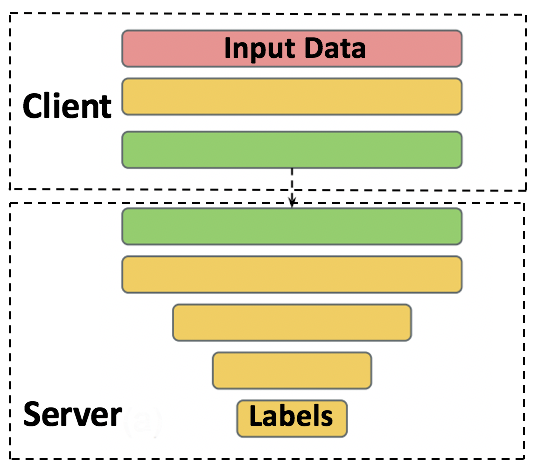
\includegraphics[width=5cm]{split_learning_vanilla.png} }}%
    \qquad
    \subfloat[U-shaped split learning]{{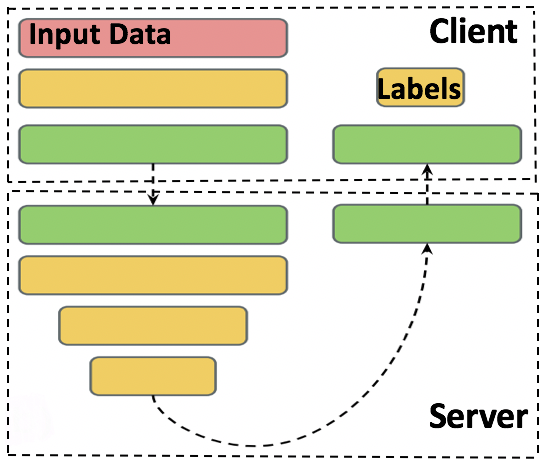
\includegraphics[width=5cm]{split_learning_U_shaped.png} }}%
    \caption{Split learning configurations showing raw data is not transferred in the vanilla setting and that raw data as well as labels are not transferred between the client and server  entities in the U-shaped split learning setting. 显示原始数据的拆分学习配置不会在 vanilla 设置中传输,并且原始数据以及标签不会在 U 形拆分学习设置中的客户端和服务器实体之间传输。}
\label{splitConfig}
\end{figure}

In several settings, the overall communication requirements of split learning and federated learning were compared in \citep{vepakomma2019splitComm}. Split learning brings in another dimension of parallelism in the training, parallelization among parts of a model, e.g. client and server. The ideas in \citep{jaderberg2017decoupled, huo2018training}, where the authors break the dependencies between partial networks and reduced total centralized training time by parallelizing the computations in different parts, can be relevant here as well. However, it is still an open question to explore such parallelization of split learning on edge devices. Split learning also enables matching client-side model components with the best server-side model components for automating model selection as shown in the ExpertMatcher \cite{sharma2019expertmatcher}.

在几种情况下,在 \citep{vepakomma2019splitComm} 中比较了拆分学习和联邦学习的总体通信要求。拆分学习在训练中引入了另一个并行维度,即模型各部分之间的并行化,例如客户端和服务器。 \citep{jaderberg2017decoupled, huo2018training} 中的想法,作者打破了部分网络之间的依赖关系,并通过并行化不同部分的计算来减少总集中训练时间,在这里也很重要。然而,在边缘设备上探索这种分裂学习的并行化仍然是一个悬而未决的问题。拆分学习还支持将客户端模型组件与最佳服务器端模型组件进行匹配,以自动选择模型,如 ExpertMatcher \cite{sharma2019expertmatcher} 所示。

The values communicated can nevertheless, in general, reveal information about the underlying data. How much, and whether this is acceptable, is likely going to be application and configuration specific. A variation of split learning called NoPeek SplitNN \citep{vepakomma2019reducing} reduces the potential leakage via communicated activations, by reducing their distance correlation \citep{vepakomma2018supervised,szekely2007measuring} with the raw data, while maintaining good model performance via categorical cross-entropy. The key idea is to minimize the distance correlation between the raw data points and communicated smashed data. The objects communicated could otherwise contain information highly correlated with the input data if used without NoPeek SplitNN, the use of which also enables the split to be made relatively early-on given the decorrelation it provides. One other engineering driven approach to minimize the amount of information communicated in split learning has been via a specifically learnt pruning of channels present in the client side activations \citep{channelPruning}. Overall, much of the discussion in \cref{sec:privacy} is relevant here as well, and analysis providing formal privacy guarantees specifically for split learning is still an open problem.

然而,通常,所传达的值可以揭示有关基础数据的信息。多少以及这是否可以接受,可能取决于应用程序和配置。一种称为 NoPeek SplitNN \citep{vepakomma2019reducing} 的分裂学习变体通过减少它们与原始数据的距离相关性 \citep{vepakomma2018supervised,szekely2007measuring} 来减少通过交流激活的潜在泄漏,同时通过分类交叉熵保持良好的模型性能。关键思想是最小化原始数据点和传达的粉碎数据之间的距离相关性。如果在没有 NoPeek SplitNN 的情况下使用,则通信的对象可能包含与输入数据高度相关的信息,鉴于它提供的去相关性,使用 NoPeek SplitNN 还可以相对较早地进行拆分。另一种工程驱动的方法是通过对客户端激活\citep{channelPruning} 中存在的通道进行专门学习的剪枝来最小化拆分学习中传达的信息量。总体而言,\cref{sec:privacy} 中的大部分讨论也与此处相关,并且专门为拆分学习提供正式隐私保证的分析仍然是一个悬而未决的问题。

\subsection{Executive summary}
The motivation for federated learning is relevant for a number of related areas of research.

\begin{itemize}
\item Fully decentralized learning (\cref{sec:decentralized}) removes the need for a central server coordinating the overall computation. Apart from algorithmic challenges, open problems are in practical realization of the idea and in understanding of what form of trusted central authority is needed to set up the task.
\item Cross-silo federated learning (\cref{ssec:cross-silo}) admits problems with different kinds of modelling constraints, such as data partitioned by examples and/or features, and faces different set of concerns when formulating formal privacy guarantees or incentive mechanisms for clients to participate.
\item Split learning (\cref{ssec:split-learning}) is an approach to partition the execution of a model between the clients and the server. It can deliver different options for overall communication constraints, but detailed analysis of when the communicated values reveal sensitive information is still missing.
\end{itemize}


\begin{itemize}
  \item 完全分散的学习(\cref{sec:decentralized})消除了对协调整体计算的中央服务器的需要。 除了算法挑战之外,开放性问题还在于该想法的实际实现以及对设置任务所需的可信中央权威形式的理解。
  \item 跨筒仓联邦学习 (\cref{ssec:cross-silo}) 承认不同类型的建模约束存在问题,例如按示例和/或特征划分的数据,并在制定正式的隐私保证或 客户参与的激励机制。
  \item 拆分学习 (\cref{ssec:split-learning}) 是一种在客户端和服务器之间划分模型执行的方法。 它可以为整体通信约束提供不同的选项,但仍然缺少对通信值何时揭示敏感信息的详细分析。
  \end{itemize}


\pagebreak